\chapter{Graph Processing Framework}
\label{chap:c2}

The topic of Big Data has been attracting the attention in academia and industry. Extracting useful information hidden in large datasets can assist people to make better decisions. However, a single machine is often incapable to handle such large and complex datasets. Therefore the common solution is to distribute the data over the cloud and compute in parallel.

To separate distributed and parallel computation from data analytics, Google initiated MapReduce project. MapReduce offers a programming model and its associated implementation for processing large datasets\cite{dean2008mapreduce}. A MapReduce program consists of the function \emph{map} that takes an input key/value pairs and generates intermediate key/value pairs, and the function \emph{reduce} performs a merge operation on the intermediate results. It is implemented as a scalable and fault-tolerant interface. Users only need to specify the map and reduce functions, and the system executes these functions on the large datasets in a parallel fault-tolerant manner.

While the MapReduce abstraction is optimized for parallel computation on different splits of the data independently from each other, it is inefficient for graph algorithms. As MapReduce expresses a graph algorithm as a series of fine-granular MapReduce jobs, it has to pass the entire state of the graph from one stage to the next by writing data to the stable storage, which incurs much communication and serialization overhead. It also adds the programming complexity to the user. 

In addition, graph problems often exhibit the following properties that introduce challenges for efficient parallelism\cite{lumsdaine2007challenges}.

\begin{itemize}
	\item \textbf{Data-driven computations.} Computations of graph algorithms are often driven by the graph structure, while graph algorithms generally specify the computation on the vertices and edges of the graph. Therefore, parallel computation on different parts of the graph makes it difficult to partition the graph. 
	\item \textbf{Unstructured problems.} Data associated with the graph are unstructured in general, which challenge the parallelism based on partitioning the graph. Poorly partitioned graph limits the scalability and leads to workload imbalance. 
	\item \textbf{Poor locality.} Graphs describe the relationships between entities, which are often unstructured and irregular. Therefore data access shows poor locality, which limits the performance of a system.
	\item \textbf{High data access to computation ratio.} Graph algorithms often interest in exploring the information in a graph rather than computation intensive processing on graph data. Frequently data access with poor locality will result in long latency.
\end{itemize}

Graph analytics becomes increasingly important with trend of Big Data for solving many problems in widely range. In order to address the challenge of graph algorithms to MapReduce-based frameworks, researchers proposed graph processing frameworks such as Pregel\cite{malewicz2010pregel} and PowerGraph\cite{gonzalez2012powergraph}. These frameworks provide users with an interface to specify their algorithms in a vertex-centric program, in which each vertex generally gathers data from its neighbors, updates its own data and informs neighbors about the change. Frameworks distribute the graph over cluster, execute the vertex-centric program on each vertex in a parallel manner and provide fault-tolerant. In contrast to MapReduce, these frameworks keep states of the graph, i.e. vertices and edges, during the computation.

\section{Pregel}

Pregel is a scalable and fault-tolerant general-purpose platform on which large scale graphs can be processed in a distributed environment. The API provided by Pregel is sufficient to implement many graph algorithms over arbitrary graph representations, and hides the details of distribution, such as message passing and fault tolerance.

\subsection{Computation Model}

The input graph to Pregel is a directed graph. Each vertex has a unique identifier and is associated with mutable user-defined data. Each edge is associated to its source vertex and mutable user-defined data. As there are lots of file formats of graphs, Pregel allows user to define how to interpret an file to the input graph.

Pregel follows the Bulk Synchronous Parallel (BSP) model\cite{valiant1990bridging}, which defines the synchronous computation and communication. The computation in Pregel is associated with vertices, which consists of a sequence of iterations, namely \textit{superstep}. Initially all the vertices are activated by the framework, and all active vertices are involved in the computation in any given superstep. Within each superstep, each vertex in parallel receives the message sent to it in the last superstep and invokes the same user-defined vertex function. The vertex function specifies the behavior according to the graph algorithm at a single vertex in a superstep, which can modify the data associated with the vertex and send messages to other vertices. A vertex decides to halt and becomes inactive when there is no further work to do, but it can be reactivated externally by the messages from others. If a vertex is in the inactive state, the framework will not execute the vertex function in the next superstep. The program terminates when all vertices decide to halt and no message in transit.

A vertex can send messages directly to others, even if the target vertex is not a neighbor. The message consists of a user-defined value and the destination vertex. The messages sent in current superstep are guaranteed to be delivered in the next superstep and not duplicated. The vertex function in Pregel is even allowed to modify the topology of the graph.

When the destination vertex of a message is on another machine, communication overhead is incurred, which might be reduced in some cases. For example, in the PageRank algorithm, received floating valued messages are summed up and then used in the vertex function. The messages sent to a same vertex can be combined to one message to reduce the overhead, if the combination operation is commutative and associative. Because the sequence of performing combination operation does not effect the final result.

Pregel also provides \textit{aggregators} for statistics and global coordination. Each vertex can submit a value to an aggregator in a superstep, and the aggregator combines these values to a single one, which is available in the next superstep. For example, a serial of different computations are performed over supersteps, and an aggregator decides to move to next computation when all vertices have fulfilled some requirements.

The output of the framework is the data generated by the vertices. Generally it is the same directed graph as input, but some algorithms would add or remove vertices or edges during the computation.

\subsection{Pregel Achitecture}

Pregel was designed to run on the Google cluster architecture. Each cluster has thousands of PCs. Pregel divides a graph into partitions, each of which contains a set of vertices and their associating out-going edges. A random hash by default is applied to assign a vertex to a partition. This will affect the performance, as many algorithms can benefit from a heuristic partitioning.

Basically a Pregel program executes like following. Many copies of the program start on a cluster. One of these is chosen as the master, which only coordinates the execution. The others, namely workers, register themselves to the master. The master determines the partitions and assigns one or more partitions to each worker. Each worker loads a part of the graph assigned by the master, maintains the state of the graph, executes vertex function and manages sending and receiving messages. The master instructs the workers to perform a superstep and waits for the response from the workers.

Pregel implements fault tolerance by \textit{checkpointing}. The workers save their partitions to stable storage, including vertex data, edge data, and incoming messages, and the master saves the aggregator values. The master pings the workers to detect the failure of the workers. When a worker does not receive a ping from the master after a specified period, the worker terminates the execution. When the master does not receive the response from a worker, then it deem the worker failed. When any worker fails, the master assigns the partitions in the failed workers to other available workers. They reload the partitions from the previous checkpoint and repeat the missing computations to the current superstep.

%\subsection{Performance}

%Many applications of graph algorithms, like PageRank and Shortest Path, have been implemented on Pregel framework. The experiments with the single-source shortest paths (SSSP) show that Pregel has a satisfactory performance with relatively little coding effort and a better scaling performance comparing with others.

\section{GraphLab}

In \cite{Low+al:uai10graphlab} the researchers argue that many algorithms of Machine Learning and Data Mining are characterized by asynchronous, dynamic, graph-parallel computation. Distributed GraphLab in shared-memory setting is presented to provide a high-level distributed abstraction for those algorithms.

\subsection{Computation Model}

The computation model of GraphLab has three major parts, the data graph, the update function and the sync operation. The data graph is similar to the one in Pregel. In GraphLab the program state and user-defined data $D$ are directly stored in the data graph $G=(V,E,D)$. Users are allowed to associate any data with vertices $\{D_v: v \in V\}$ and edges $\{D_{u \leftrightarrow v}: \{u,v\} \in E\}$. It is important to notice that GraphLab does not distinguish the directions of edges. Although the graph data can be modified, the structure of the graph is not allowed to be changed during execution. 

The update function $f(v,S_v) \rightarrow (S_v, T)$, which is a synonym of the vertex function, takes the data within the scope $S_v$ of a vertex $v$ as input, and returns the updated data and the scheduled vertices $T$ for further execution. The scope of a vertex includes the vertex and its adjacent edges and vertices as well as the associated data, as shown in Figure~\ref{fig:Scope}. The dashed rectangle marks the scope of vertex 3. The update function on vertex 3 can read and write all data in $S_3$, which includes vertex data $D_2, D_3, D_4$ and edge data $D_{2 \leftrightarrow 3}, D_{3 \leftrightarrow 4}$.

\begin{figure}[H]
  \begin{center}
    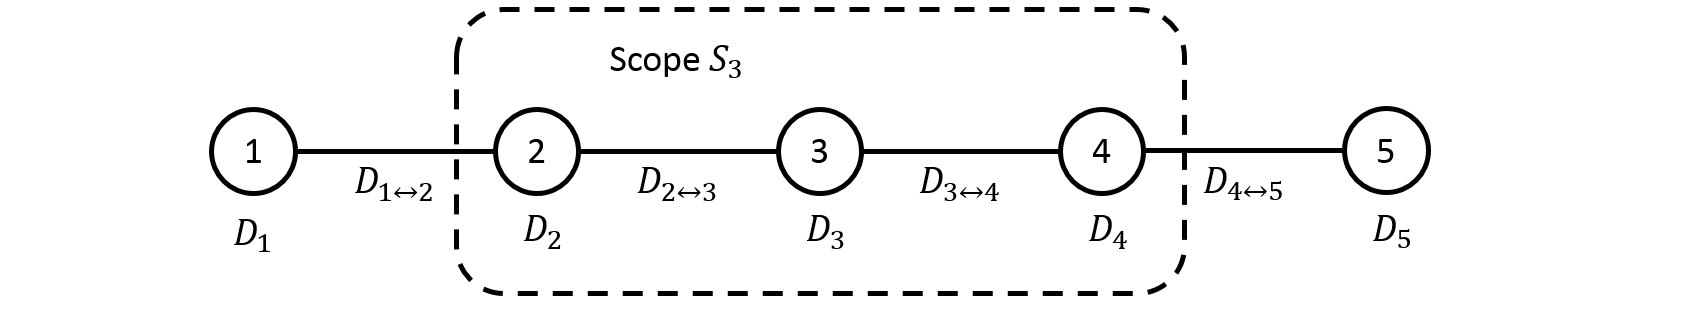
\includegraphics[width=\textwidth]{Scope.png}
    \caption{Scope $S_3$ of vertex 3}
    \label{fig:Scope}
  \end{center}
\end{figure}

In contrast to Pregel, in which the execution of vertex function is triggered by the messages and can access the data only in the messages, GraphLab separates the movement of the data and scheduling for execution. Therefore update function in GraphLab can access data of adjacent vertices even if the vertices are not scheduled. The update function in GraphLab gives user freedom to access the data of adjacent edges and vertices. By returning the scheduled vertices, GraphLab is able to express dynamic computation. 

Algorithm~\vref{alg:GraphLabExecutionModel}\cite{Low+al:uai10graphlab} shows the GraphLab execution model. The input to GraphLab are the data graph $G=(V,E,D)$ and an initial vertex set $T$ that are scheduled when the execution starts (line 1-2). While there exist vertices in the set $T$ (line 3), a vertex is removed from the set and the update function is executed, which updates the data within the scope and returns a set of scheduled vertices (line 4-5). The vertex set $T$ is updated, in which duplicated vertices are ignored (line 6). The output is the updated data graph. 

	\begin{Algorithmus}[H]
	\label{alg:GraphLabExecutionModel}
	\caption{GraphLab Execution Model}	
	\begin{algorithmic}[1]
	\State \textbf{Input}: Data Graph $G=(V,E,D)$
	\State \textbf{Input}: Initial vertex set $T$
	\While{$T \neq \emptyset$}
		\State $v \leftarrow RemoveNext(T)$
		\State $(S_v, T') \leftarrow f(v,S_v)$
		\State $T \leftarrow T \cup T'$
	\EndWhile
	\State \textbf{Output}: Modified Data Graph $G=(V,E,D')$
	\end{algorithmic}	
	\end{Algorithmus}

Due to asynchronous parallel execution in GraphLab, it must be avoided that update function of different vertices modify the data simultaneously. Otherwise, race condition may lead to non-deterministic behaviour. For example, non-deterministic happens, when both vertex 3 and vertex 4 in Figure~\ref{fig:Scope} try to write $D_{3 \leftrightarrow 4}$ in parallel. A serializable execution avoids executing overlapping computation at the same time. A serializable execution in GraphLab means that the scheduled parallel execution by Algorithm~\vref{alg:GraphLabExecutionModel} has a corresponding serial execution of update function that produces the same result. Therefore GraphLab introduces three consistency models as shown in Figure~\ref{fig:ConsistencyModel}. The full consistency model ensures each update function has exclusive read-write access to the vertex scope. The edge consistency ensures each update function has exclusive read-write access to the vertex and adjacent edges but read only access to adjacent vertices. The vertex consistency ensures each update function has exclusive read-write access to the vertex but read only access to adjacent edges. From full consistency to vertex consistency, the consistency degree is decreasing while the parallelism degree is increasing.

\begin{figure}[H]
  \begin{center}
    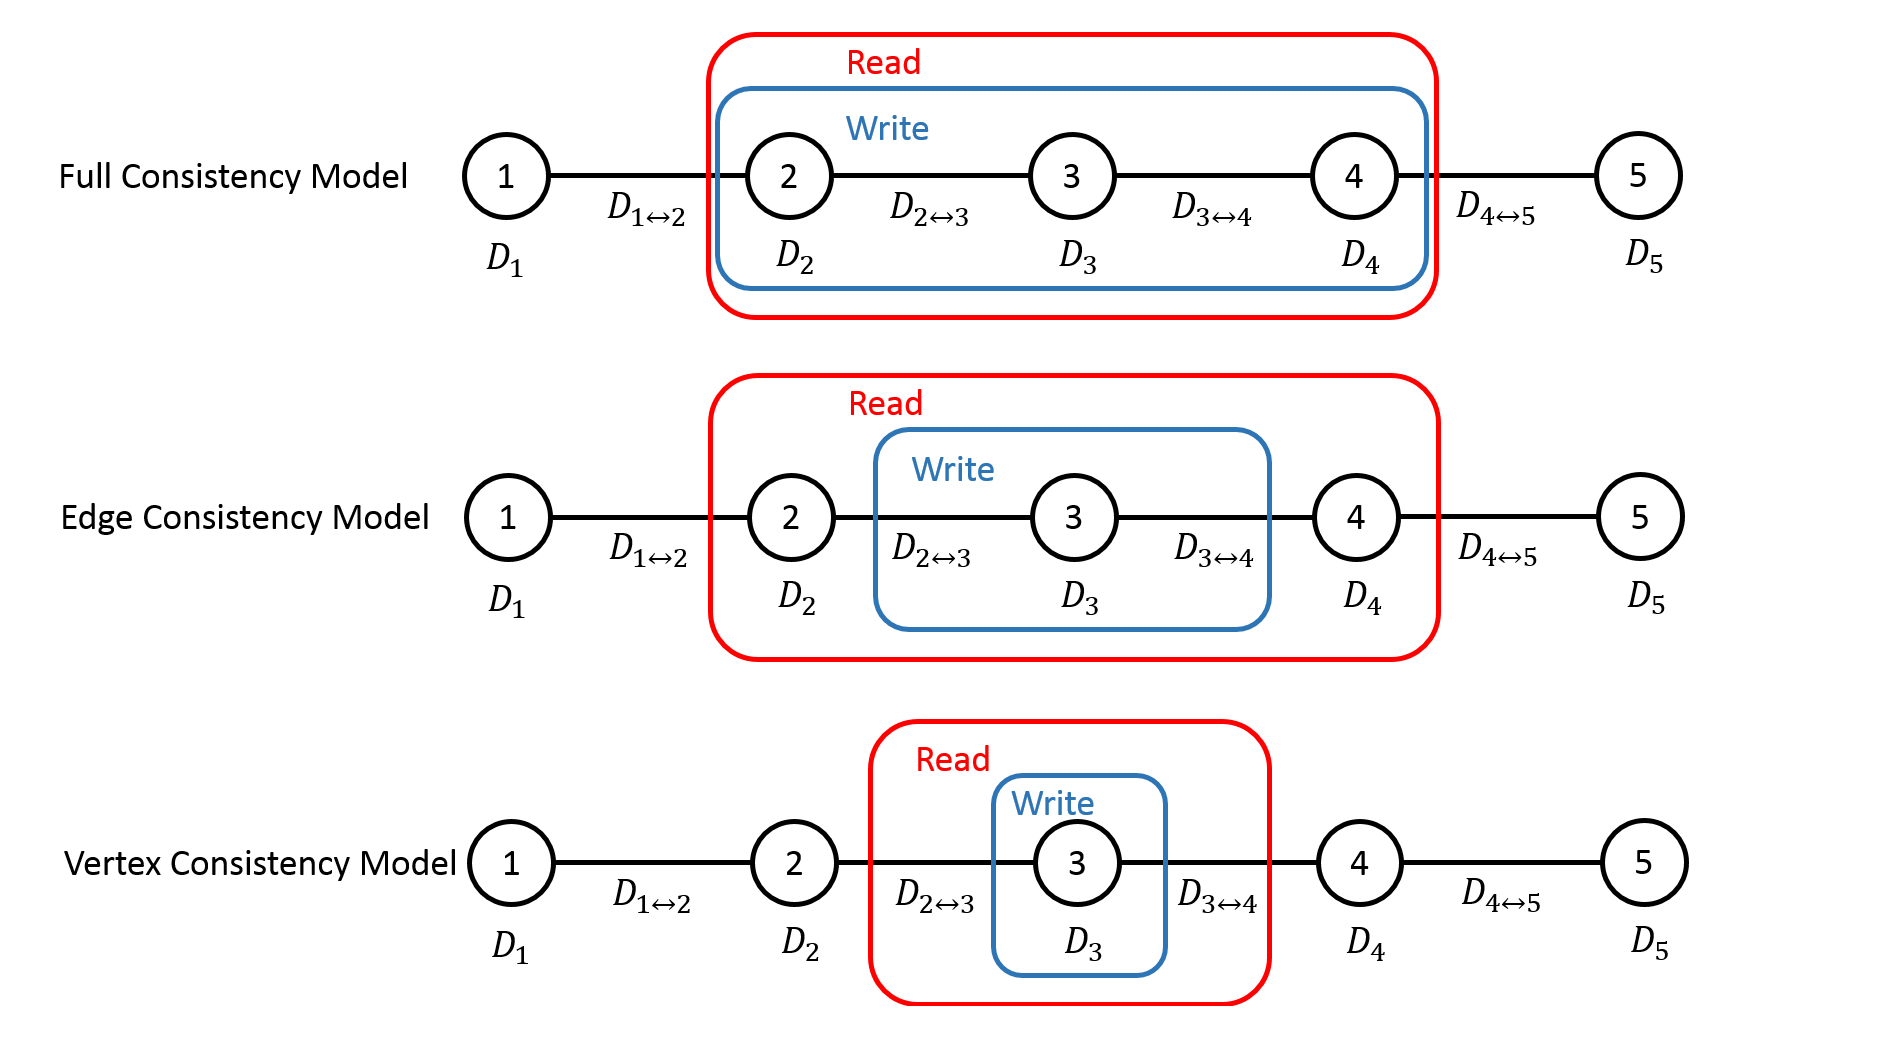
\includegraphics[width=\textwidth]{ConsistencyModel.png}
    \caption{Consistency models}
    \label{fig:ConsistencyModel}
  \end{center}
\end{figure}

The sync operation is similar to the aggregator in Pregel. In contrast to the aggregator, the sync operation has a finalization phase and runs continuously.

\subsection{Distributed GraphLab Architecture}

GraphLab uses a graph representation based on two-stage partitioning, which is efficient and balance to load graph on the cluster. Firstly the data graph is partitioned into many small pieces using domain specific knowledge or partitioning heuristic, which is much greater than the number of machines. Each piece is called an atom and stored separately on the distributed storage. The atom also stores the ghosts, which are the set of vertices and edges adjacent to the boundary. A meta-graph is created, in which vertices represent atoms. In second stage, GraphLab loads the meta-graph and distributes atoms over machines by a fast balanced partition. This technique allows the re-usage of graph partition.

GraphLab introduces two approaches to implementing the execution model. The \textit{Chromatic Engine} uses graph coloring that assigns each vertex with a color so that no adjacent vertices are assigned with the same color. The edge consistency is satisfied, when executing simultaneously all vertices of same color with a graph coloring. Other consistency model can also be satisfied by changing graph coloring. However the Chromatic Engine is not sufficient to flexibly schedule in many cases. The \textit{Locking Engine} extends the mutual exclusion in shared memory engine by associating readers-writer lock with each vertex. Different consistency models are implemented with different protocols.

GraphLab uses two approaches to creating snapshot for fault tolerance. To create a synchronous snapshot, execution is suspended, communication channels are flushed and all the data are saved to file-system. Asynchronous approach is based on the Chandy-Lamport snapshot, as the machines and channels in the Chandy-Lamport snapshot can be replaced by vertices and edges. The experiments also show that the asynchronous snapshot only slows down the execution, while the synchronous snapshot stops the execution.

\section{PowerGraph}

In \cite{gonzalez2012powergraph} the researchers point out that the natural graphs in the real world are characterized by highly skewed power-law degree distribution, which means most vertices have a few neighors while a few vertices have many neighbors. The probability of a vertex having degree $d$ under power-law distribution is:

\begin{equation}\label{eq:PowerLawDegree}
P(d) \propto d^{-\alpha}
\end{equation}

where $\alpha$ is a positive constant. In a highly skewed graph, the edges concentrate on a small fraction of vertices, which challenges the graph processing frameworks. The power-law degree distribution leads to partitioning difficulty and imbalance of communication, computation and storage. PowerGraph is proposed to address these problems by exploiting the characterization of the graph programs and the structure of the power-law graphs.

\subsection{The GAS Computation Model}

PowerGraph summarized the common features of the vertex function that are shared by both Pregel and GraphLab, and introduces the GAS model to characterize generality and differentiate the computation of vertices and edge. The GAS model represents three phase of a vertex function: \textbf{G}ather, \textbf{A}pply and \textbf{S}catter. 

PowerGraph offers an interface to implement algorithms in GAS model, which is shown in Figure~\ref{fig:GASVertexFunction} \cite{gonzalez2012powergraph}. The gather function is invoked on a set of adjacent edges of the vertex $u$ in parallel. The set of edges can be \emph{none}, \textit{in}, \textit{out} or \textit{all}, which is determined by \textit{gather\_nbrs}. The gather function collects the data and returns a temporary accumulator, which is then fed to the sum function to produce a final result $Accum$. The sum function inherits the commutative and associative gather concept from Pregel.

Based on the old vertex data $D_u$, the apply function uses the final result $Accum$ to update new vertex data $D^{new}_u$ which is saved to the graph by an atomic operation. The size of the accumulator $Accum$ and complexity of the apply function play a central role in determining the network and storage efficiency of the PowerGraph abstraction.
 
The scatter function is invoked on a set of adjacent edges determined by \textit{scatter\_nbrs}, which is same as in gather function. The scatter function may also update the data of the adjacent edges.

\begin{figure}
  \begin{center}
    
\includegraphics[width=\textwidth]{GASVertexFunction.png}
    \caption{GAS vertex function interface}
    \label{fig:GASVertexFunction}
  \end{center}
\end{figure}


%In the gather phase, the vertex gathers the information from adjacent edges and vertices. Then a commutative and associative sum operation $\oplus$ is performed on the gathered data:

%$$\forall v \in Nbr[u]: Accum \leftarrow \oplus gather(D_u,D_{(u,v)},D_v)$$

%The resulting data $Accum$ is used in apply phase to update the data of the current vertex. 

%$$D^{new}_u \leftarrow a(D_u,Accum)$$

%In the scatter phase, the new vertex data is used to update the data of adjacent edges.

%$$\forall v \in Nbr[u]: D_{(u,v)} \leftarrow scatter(D^{new}_u,D_{(u,v)},D_v)$$

A vertex becomes inactive after completion of the scatter phase but can be reactivated. A vertex can activate itself and the neighboring vertices. For example, in the PageRank a vertex gathers data from in-edges and uses the summed result to update its value and operates on out-edges in scatter phase. Further activation of vertices can be done in any GAS functions, but only the vertices that are visible in the specific function arguments. For example, a vertex can activate itself in apply function and neighbors in scatter function.

In Pregel and GraphLab abstraction the GAS model is expressed differently. Pregel uses message passing and combiner instead of the gather phase, and implements the apply phase and the scatter phase within vertex function. GraphLab allows user-defined vertex function to access entire information within the neighborhood.

\subsection{PowerGraph Architecture}

PowerGraph divides the vertex function into GAS model, so that it can express an algorithm in "think-like-a-vertex", and distribute the computation of a single vertex function over the cluster. %It inherits the commutative associative gather concept from Pregel and also borrows the data graph and shared-memory to keep user from specifying the data movement.
In addition, a vertex might be activated while a few of its neighbors are changed. However, the gather function is invoked on all neighbors. Therefore the gather function can be skipped for some algorithms by caching the accumulator and updating the accumulator with an optional $\Delta a$ returned by the scatter function. If the scatter function does not return $\Delta a$, then the cached accumulators of neighbors are cleared to force a complete gather phase on neighbors in next execution.

Algorithm~\vref{alg:PowerGraphExecutionModel} \cite{gonzalez2012powergraph} expresses the semantics how PowerGraph engine invokes GAS functions. The gather function is skipped if cached accumulator is empty. Otherwise the gather function is performed (line 2-6). The apply function uses the accumulator for update (line 7). In the scatter function, an optional returned $\Delta a$ is used to update the accumulator of each neighboring vertex, when both $\Delta a$ and neighboring accumulator are not empty. Otherwise, neighboring accumulator is set to empty (line 8-15).

	\begin{Algorithmus}[H]
	\label{alg:PowerGraphExecutionModel}
	\caption{PowerGraph Execution Model}	
	\begin{algorithmic}[1]
	\State \textbf{Input}: Center vertex $u$
	\If{cached accumulator $a_u$ is $empty$}
		\For{neighbor $v$ in $gather\_nbrs(u)$}
			\State $a_u \leftarrow sum(a_u,gather(D_u,D_{(u,v)},D_v))$
		\EndFor
	\EndIf
	\State $D_u \leftarrow apply(D_u,a_u)$
	\For{neighbor $v$ in $scatter\_nbrs(u)$}
		\State $(D_{(u,v)}, \Delta a) \leftarrow scatter(D_u,D_{(u,v)},D_v)$
		\If{$a_v$ and $\Delta a$ are not $empty$}
			\State $a_v \leftarrow sum(a_v, \Delta a)$
		\Else
			\State $a_v \leftarrow empty$
		\EndIf
	\EndFor	
	\end{algorithmic}	
	\end{Algorithmus}

The execution order of activated vertices depends on The PowerGraph engine. PowerGraph provides both synchronous engine and asynchronous engine. The synchronous engine executes each phase in order on all active vertices, which is synchronized with a barrier at the end of each phase. A superstep is defined as a complete series of GAS functions. The changes made in each phase are visible in the next phase. Vertices activated in each superstep are executed in the next superstep. Synchronous execution is similar to Pregel, which ensures a deterministic execution but limits the parallelism of the algorithms. The asynchronous engine can efficiently execute active vertices as long as resources are available, which accelerates the convergence of some algorithms. The changes on data of edges and vertices are immediately visible to neighbors in following computation. The asynchronous execution leads to non-deterministic, which is not suitable for some algorithms and is difficult for debugging. To retain the strong serializability, PowerGraph improves the locking protocol proposed in GraphLab, which is fair to high degree vertices. 

\subsection{Vertex Cut}

One way to place a graph on $p$ different machines is the balanced $p$-way edge-cut, which evenly assigns the vertices to different machine and minimizes the the number of edges spanning over machines. However, it does not work well with power-law graphs. Frameworks like Pregel and GraphLab usually use random hash to place vertices, which is easy and fast, but cuts most of the edges. Every spanning edge exacerbates the overhead of storage and communication, because both machines have to maintain a copy of the adjacent data and synchronize the data.

To reduce communication and balance workload, PowerGraph uses vertex cut to place the graph. Similarly a $p$-way vertex-cut evenly assigns edges to $p$ machines and aims at minimizing the number of vertices spanning over multiple machines. Figure~\ref{fig:EdgeCutVertexCut} demonstrates edge-cut and vertex-cut, which partitions the graph over two machines. The dashed vertices are the mirrors. The two-way edge-cut yields three vertices that are replicated on the two machines, while the two-way vertex-cut only yields one.

\begin{figure}
  \begin{center}
    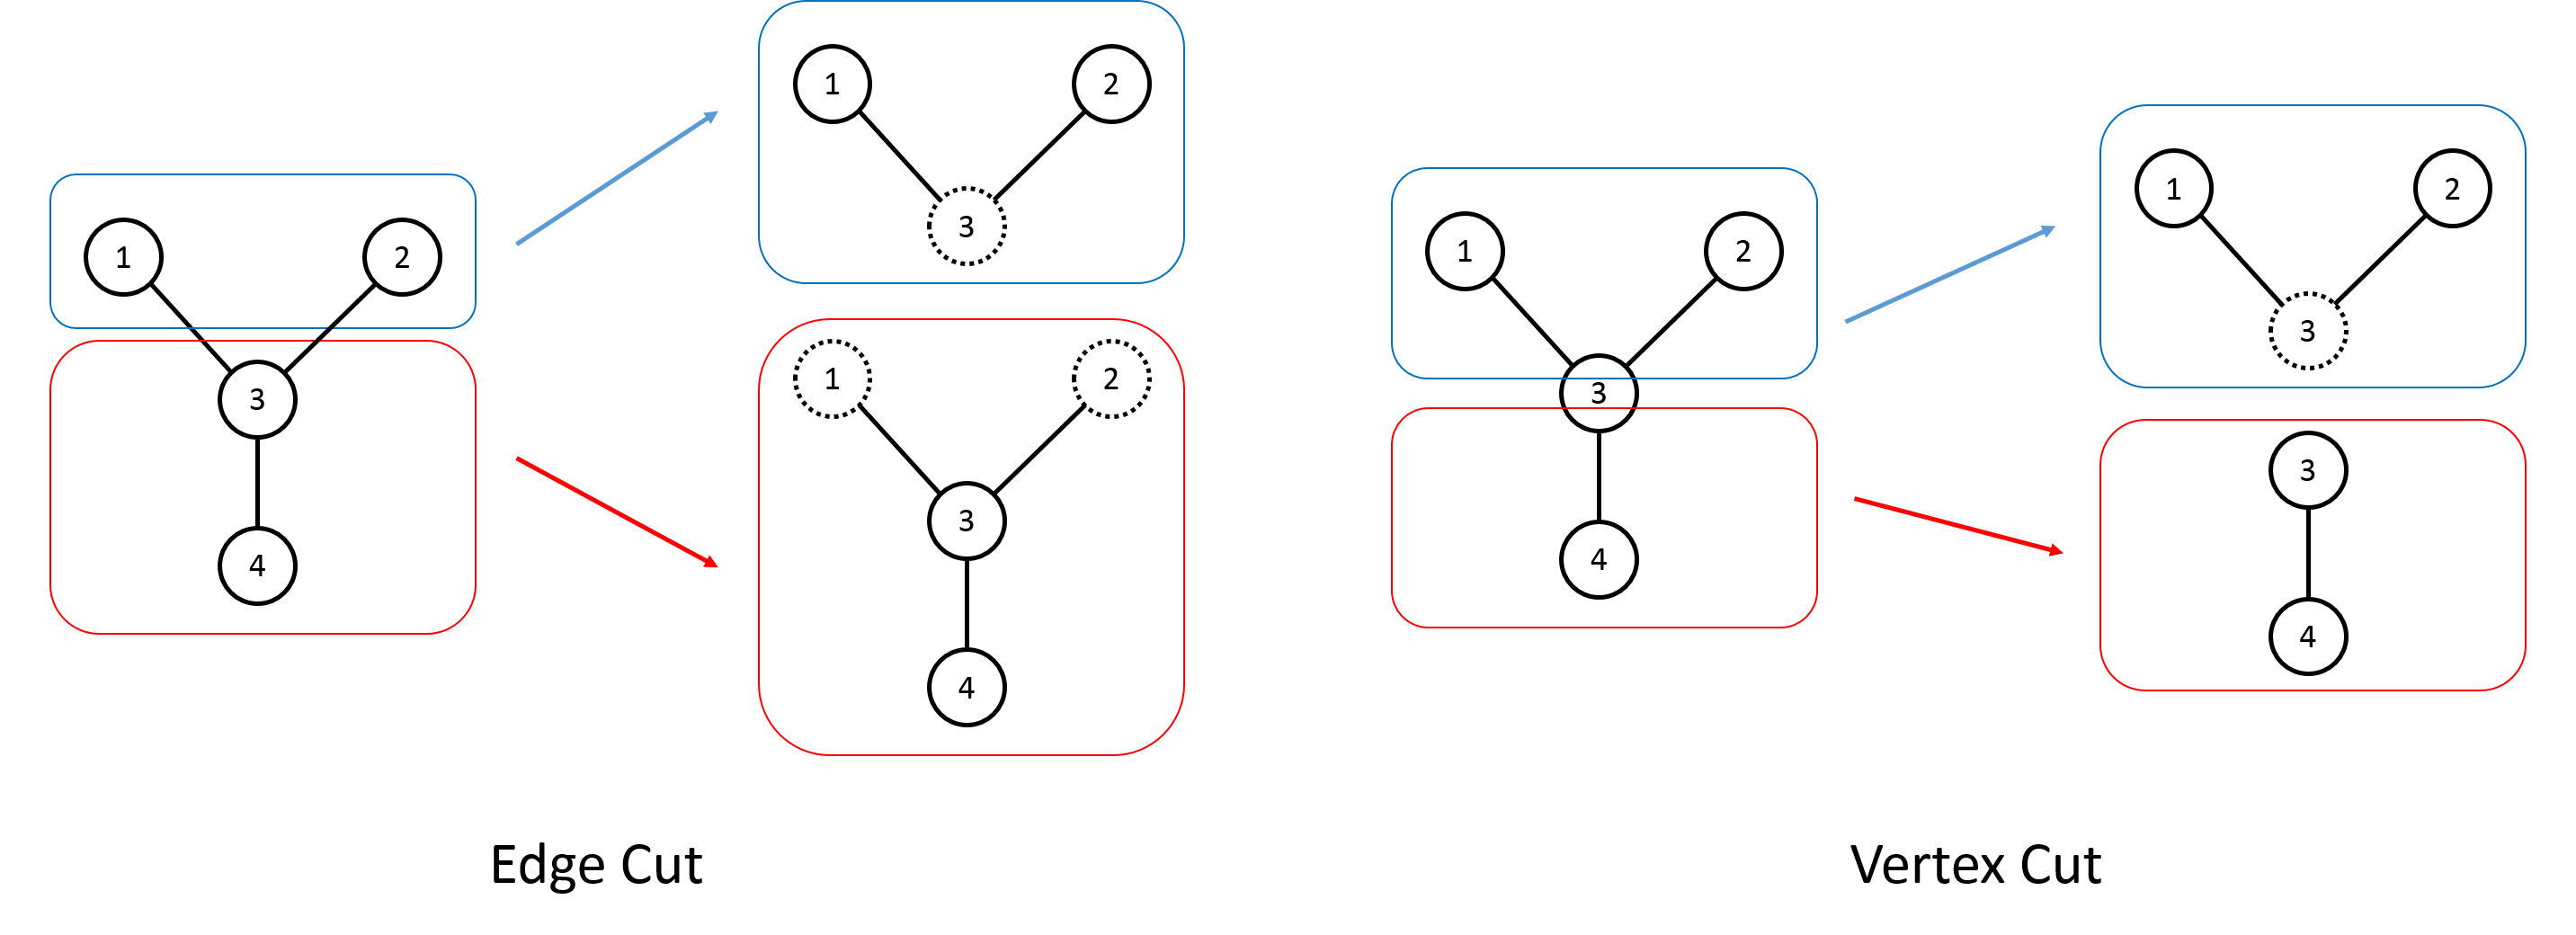
\includegraphics[width=\textwidth]{EdgeCutVertexCut.png}
    \caption{Demonstration of edge-cut and vertex-cut}
    \label{fig:EdgeCutVertexCut}
  \end{center}
\end{figure}

Therefore PowerGraph abstraction allows vertex as well as its vertex function to span over machines. Figure~\ref{fig:SplitVertexFunction} shows that a vertex function is split over two machines. The rectangles of gather, apply and scatter functions represent their execution region. By using vertex cut, massive edges are distributed over machines and each edge is stored on only one machine. Therefore modifications on edge data do not need communication. But modifications on vertex data must be committed to all the machine it spans. Therefore the number of machines that vertices span determines the storage and communication overhead.

\begin{figure}
  \begin{center}
    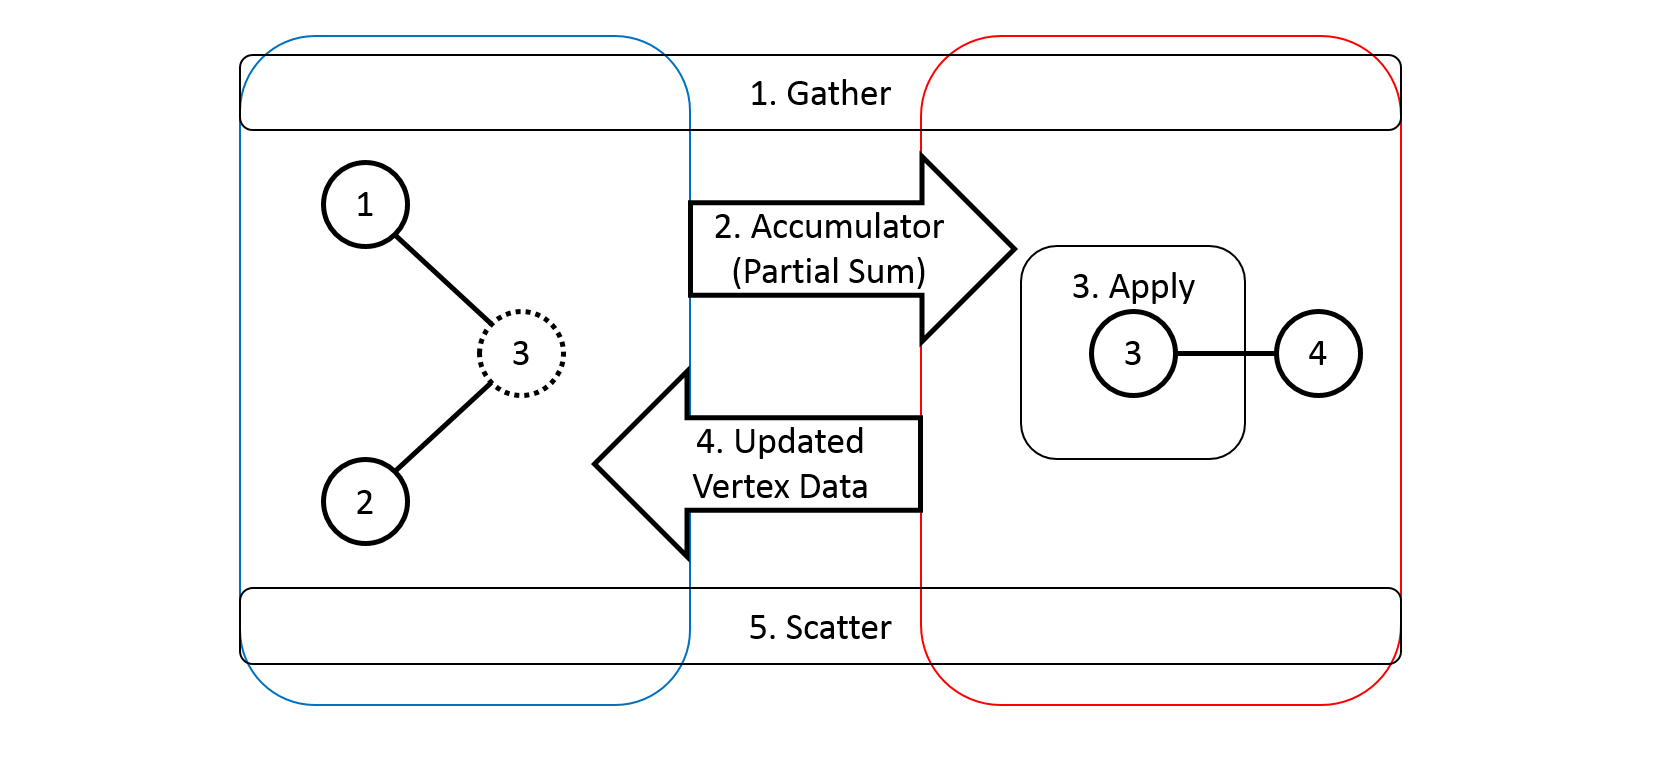
\includegraphics[width=\textwidth]{SplitVertexFunction.png}
    \caption{Vertex function that is split over two machines}
    \label{fig:SplitVertexFunction}
  \end{center}
\end{figure}


The term \textit{replicas} is used to denote the set of machines that a vertex spans. One of the replicas is randomly chosen as the \textit{master} that maintains the master version of the vertex data. The rest replicas are mirrors that only keeps a local copy of the vertex data. Modifications on the vertex data during apply phase are first made to the master and then copied to all mirrors.

Randomly assigning edges to machines is the simplest way to construct a vertex cut, which is completely data-parallel and can achieve a satisfactory result. Greedy-heuristic can be used to improve the result. Greedy-heuristic performs a sequential edge assignment by assigning the next edge on the machine which can minimize the conditional expected replication factor. Greedy-heuristic gives a result that is theoretically no worse than random edge assignment and often better in practice. However, greedy-heuristic needs coordination between machines. PowerGraph offers two implementations for the greedy-heuristic. In \textit{Oblivous}, each machine runs the greedy-heuristic independently and estimates replication factor locally. In \textit{Coordinated}, each machine communicates periodically on previous edge assignment to estimate replication factor.

The experiments show that greedy-heuristic results in a smaller replication factor than random placement, but with longer ingress time. The runtime scales linearly with replication factor. Therefore the greedy-heuristic improves overall runtime when PageRank has more than 20 iterations in the experiment.

\section{Other Graph Processing Frameworks}

There exist many other systems for graph processing, which are often based on a existing framework, and overcome some limitations or improve the performance. For example, GPS (for Graph Processing System)\cite{salihoglu2013gps} is similar to Pregel, while it features a dynamic repartitioning method during the execution. GPS is also optimized for skewed graphs by distributing adjacency lists of high-degree vertices across all machines.

In GraphX\cite{xin2013graphx} researchers argue that graph processing frameworks often have shortage in graph construction and transformation, so the following computations could be problematic. GraphX combines the best of both graph-parallel systems and data-parallel systems by using resilient distributed datasets to express graph computation efficiently. The Resilient Distributed Graph (RDG) was presented as a graph abstraction, which supports many operation on a graph. It uses a tabular data representation for the efficient vertex-cut partitioning. 

PowerLyra\cite{chen2015powerlyra} is motivated by the observation that most graph processing frameworks treat and process all vertices uniformly. This would incur imbalance of workload or communication for either high-degree vertices or low-degree vertices. Therefore PowerLyra introduces a computation engine that supports dynamic differentiated processing according to vertex degree. It also provides a balanced $p$-way hybrid-cut strategy with heuristics for efficient graph partitioning, which combines the best of edge-cut and vertex-cut. To improve the data access locality, PowerLyra proposes locality-conscious graph layout. As PowerLyra is implemented based PowerGraph, the algorithms designed on PowerGraph can be seamlessly executed on PowerLyra.


%The parallel BGL\cite{gregor2005parallel}

%GraphChi\cite{kyrola2012graphchi}

%Mizan\cite{khayyat2013mizan}